\documentclass[a4paper, 12pt]{article}

%%%%%%%%%%%%
% Packages %
%%%%%%%%%%%%

\usepackage[english]{babel}
\usepackage[noheader]{packages/sleek}
\usepackage{packages/sleek-title}
\usepackage{packages/sleek-theorems}
\usepackage{packages/sleek-listings}
\usepackage{verbatim}
\usepackage{listings}
\usepackage{xcolor}
\definecolor{mygreen}{rgb}{0,0.6,0}
\definecolor{mygray}{rgb}{0.5,0.5,0.5}
\definecolor{mymauve}{rgb}{0.58,0,0.82}
\lstset{ 
  backgroundcolor=\color{white},   % choose the background color; you must add \usepackage{color} or \usepackage{xcolor}; should come as last argument
  basicstyle=\ttfamily\scriptsize,        % the size of the fonts that are used for the code
  breakatwhitespace=false,         % sets if automatic breaks should only happen at whitespace
  breaklines=true,                 % sets automatic line breaking
  captionpos=b,                    % sets the caption-position to bottomhttps://www.overleaf.com/project/5e8f247c51e4ab0001a4aad8
  commentstyle=\color{mygreen},    % comment style
  deletekeywords={},            % if you want to delete keywords from the given language
  escapeinside={},          % if you want to add LaTeX within your code
  extendedchars=true,              % lets you use non-ASCII characters; for 8-bits encodings only, does not work with UTF-8
  firstnumber=1000,                % start line enumeration with line 1000
  frame=none,	                   % adds a frame around the code
  keepspaces=true,                 % keeps spaces in text, useful for keeping indentation of code (possibly needs columns=flexible)
  columns=fullflexible,
  keywordstyle=\color{black},       % keyword style
  language=python,                 % the language of the code
  morekeywords={*,...},            % if you want to add more keywords to the set
  numbers=none,                    % where to put the line-numbers; possible values are (none, left, right)
  numbersep=5pt,                   % how far the line-numbers are from the code
  numberstyle=\tiny\color{mygray}, % the style that is used for the line-numbers
  rulecolor=\color{black},         % if not set, the frame-color may be changed on line-breaks within not-black text (e.g. comments (green here))
  showspaces=false,                % show spaces everywhere adding particular underscores; it overrides 'showstringspaces'
  showstringspaces=false,          % underline spaces within strings only
  showtabs=false,                  % show tabs within strings adding particular underscores
  stepnumber=2,                    % the step between two line-numbers. If it's 1, each line will be numbered
  stringstyle=\color{mymauve},     % string literal style
  tabsize=5,	                   % sets default tabsize to 2 spaces
  title=\lstname                   % show the filename of files included with \lstinputlisting; also try caption instead of title
}
\hypersetup{
    colorlinks = true,
    linkcolor = black,
    anchorcolor = black,
    citecolor = black,
    filecolor = black,
    urlcolor = black
    }
\usepackage{longtable}

%%%%%%%%%%%%%%
% Title-page %
%%%%%%%%%%%%%%

\logo{./resources/image/logo.png}
\institute{Polytechnic of Turin}
\faculty{Computer engineering}
\department{Department of Computer Engineering, \linebreak Cinema and Mechatronics}
\title{Real-Time Sign Language Detection Bound By User Attention Recognition }
\subtitle{Course of Computer Vision and Image Processing}
\author{\textit{s281657} Angela \textsc{D'Antonio}\linebreak
        \textit{s281330} Federica \textsc{Moro}\linebreak
        \textit{s286312} Marzio \textsc{Vallero}\linebreak}

\supervisor{Professors\linebreak
            Bartolomeo \textsc{Montrucchio}\linebreak
            Luigi     \textsc{De Russis}\linebreak}

\date{a.y. 2020/2021}

%%%%%%%%%%%%%%%%
% Bibliography %
%%%%%%%%%%%%%%%%

%%%%%%%%%%
% Others %
%%%%%%%%%%
\lstdefinestyle{latex}{
    language=TeX,
    style=default,
    %%%%%
    commentstyle=\ForestGreen,
    keywordstyle=\TrueBlue,
    stringstyle=\VeronicaPurple,
    emphstyle=\TrueBlue,
    %%%%%
    emph={LaTeX, usepackage, textit, textbf, textsc}
}

\FrameTBStyle{latex}

\def\tbs{\textbackslash}

\usepackage[nottoc]{tocbibind}

%%%%%%%%%%%%
% Document %
%%%%%%%%%%%%

\begin{document}
\maketitle
\romantableofcontents
\sloppy
\twocolumn

\section{Abstract}
\label{Abstract}
This paper describes all the theoretical and implementation aspects regarding the generation of a neural network to be used as means for recognizing the alphabet of the Italian sign language.
The first part describes the software libraries and techniques used, alongside others which were ultimately discarded.
We later describe in depth the dataset generation and labeling process and its fundamental role in increasing the final network's detection stability, without incurring in the overfitting and underfitting problems.
The training process is performed through Tensorflow's Object Detection API by taking advantage of transfer learning from a pre-trained model of Tensorflow's Model Zoo.
After that, we discuss RetinaFace, the Single-Shot Multi-Level neural network used for attention recognition, which acts as a barrier for gesture recognition, such that any gesture input is ignored when not detecting a user looking towards the camera.
Ultimately, the networks are tested in order to measure stability and performance.

\section{Introduction}
\label{Introduction}
Nowadays more and more people rely on automated information systems to improve everyday life.
Computer vision and image processing, alongside machine learning, aim to provide advanced tools which can also be used for programming functionalities and user interfaces which simplify interaction with machines.
Taking advantage of these resources, our project tries to imbue a machine with the ability to understand the inputs of a user which communicates through the use of sign language, in our specific case, the Italian Sign language. This alternative input method can prove to be useful in environments where a keyboard cannot be employed or would detract from the user experience, enforced in the case in which a user cannot use his or her voice to speak, for example in the case of smart home assistants for deaf people with camera interfaces, or whenever the environment presents too much background noise to allow for clear voice recognition. Moreover, the user's attention span must be measured, in order to let the machine discern intentional inputs from spurious ones coming from the user's behaviour when he or she is not trying to interact with the machine itself.
The paper focuses on explaining the steps we took to tackle this challenge. The first section, \textit{\hyperref[LibsAndTech]{Libraries and Techniques Used}}, describes in depth the various software libraries and techniques currently available in the field and the ones we chose to use, highlighting advantages and disadvantages of each one. Moreover, we talk about the related image processing projects we used as a reference.\linebreak
The subsections tackle \textit{\hyperref[DatasetCreationLabel]{Dataset creation and labelling}}, \textit{\hyperref[NeuralNetworkTraining]{Neural network training}}, \textit{\hyperref[GazeRec]{Gaze recognition}} and finally \textit{\hyperref[RTSignDetect]{Real time sign language detection}}, and include specifications with brief comments on their respective parts.\linebreak
The subsequent section, \textit{\hyperref[ResutsAndAnalysis]{Resuts and analysis}}, provides insight on the program's final behaviour, alongside comments on the accuracy of the two neural networks used and overall performance.
In last section we express our opinion about the work, the learning goals we got from this project and discuss the evolution of this branch of the Computer Vision field in the near future.\linebreak

\section{Libraries and Techniques Used}
\label{LibsAndTech}
\textit{\hyperref[https://github.com/MarzioVallero/Real-time-Sign-Language-Detection]{Real-time Sign Language Detection}} is a Python and OpenCV based project that provides all the steps required to produce and label a dataset in order to train a neural network for object recognition through transfer learning and use it to perform real time gestures recognition.
The input frame is processed in search of gestures only if a face is detected within the image frame and the predicted gaze direction of the user is toward the computer's screen.\linebreak

\subsection{Dataset creation and labelling}
\label{DatasetCreationLabel}
The neural network used for gesture recognition must first be trained on a dataset containing the gestures we wish to detect.
In order to do so, we followed the steps which are also described in the Python Notebooks \href{https://github.com/MarzioVallero/Real-time-Sign-Language-Detection/blob/master/GenerateDataset.ipynb}{GenerateDataset.ipynb} and \href{https://github.com/MarzioVallero/Real-time-Sign-Language-Detection/blob/master/LabelDatasetAndTrain.ipynb}{LabelDatasetAndTrain.ipynb}.\linebreak
The first step is responsible for the definition of the set of gestures and for automated sample capture. After defining the number of images we want to collect for each object (in our case a hand gesture), we proceed to actually capture the frames, which are automatically saved in separate directories according to their label of reference. It is recommended to produce for each label the same amount of frames and to insert a single gesture per frame. This step can be skipped if an already existing set is to be used instead.\linebreak
Then we define a label map containing the same set of labels on which we want to train the model onto.
The \textit{nImages} variable specifies how many images of a single gesture shall be taken: in our case, we chose to use ten different frames per gesture, of which seven have been used for training and three for testing, per label.
The main variance between sets of images for the same label were different spatial positions of the hand with respect to the frame.\linebreak
It's important to note that a wider dataset for each gesure will increase variance, possibly increasing accuracy and resilience of the final trained model. However, be warned that all the images of the dataset must be manually labeled, so choose wisely.

The labeling process is in fact done with \textit{\hyperref[Ref11]{LabelImg}}, a python based graphic tool that lets us to manually select a region of interest within each frame and label it according to a specific class.
This process produces, for each frame, an output \textit{.xml} file that embeds the coordinates of the region of interest and label of a specific frame. At the end of the process, we will have an \textit{.xml} for each frame of the dataset.

\begin{figure}[!h]
    \centering
    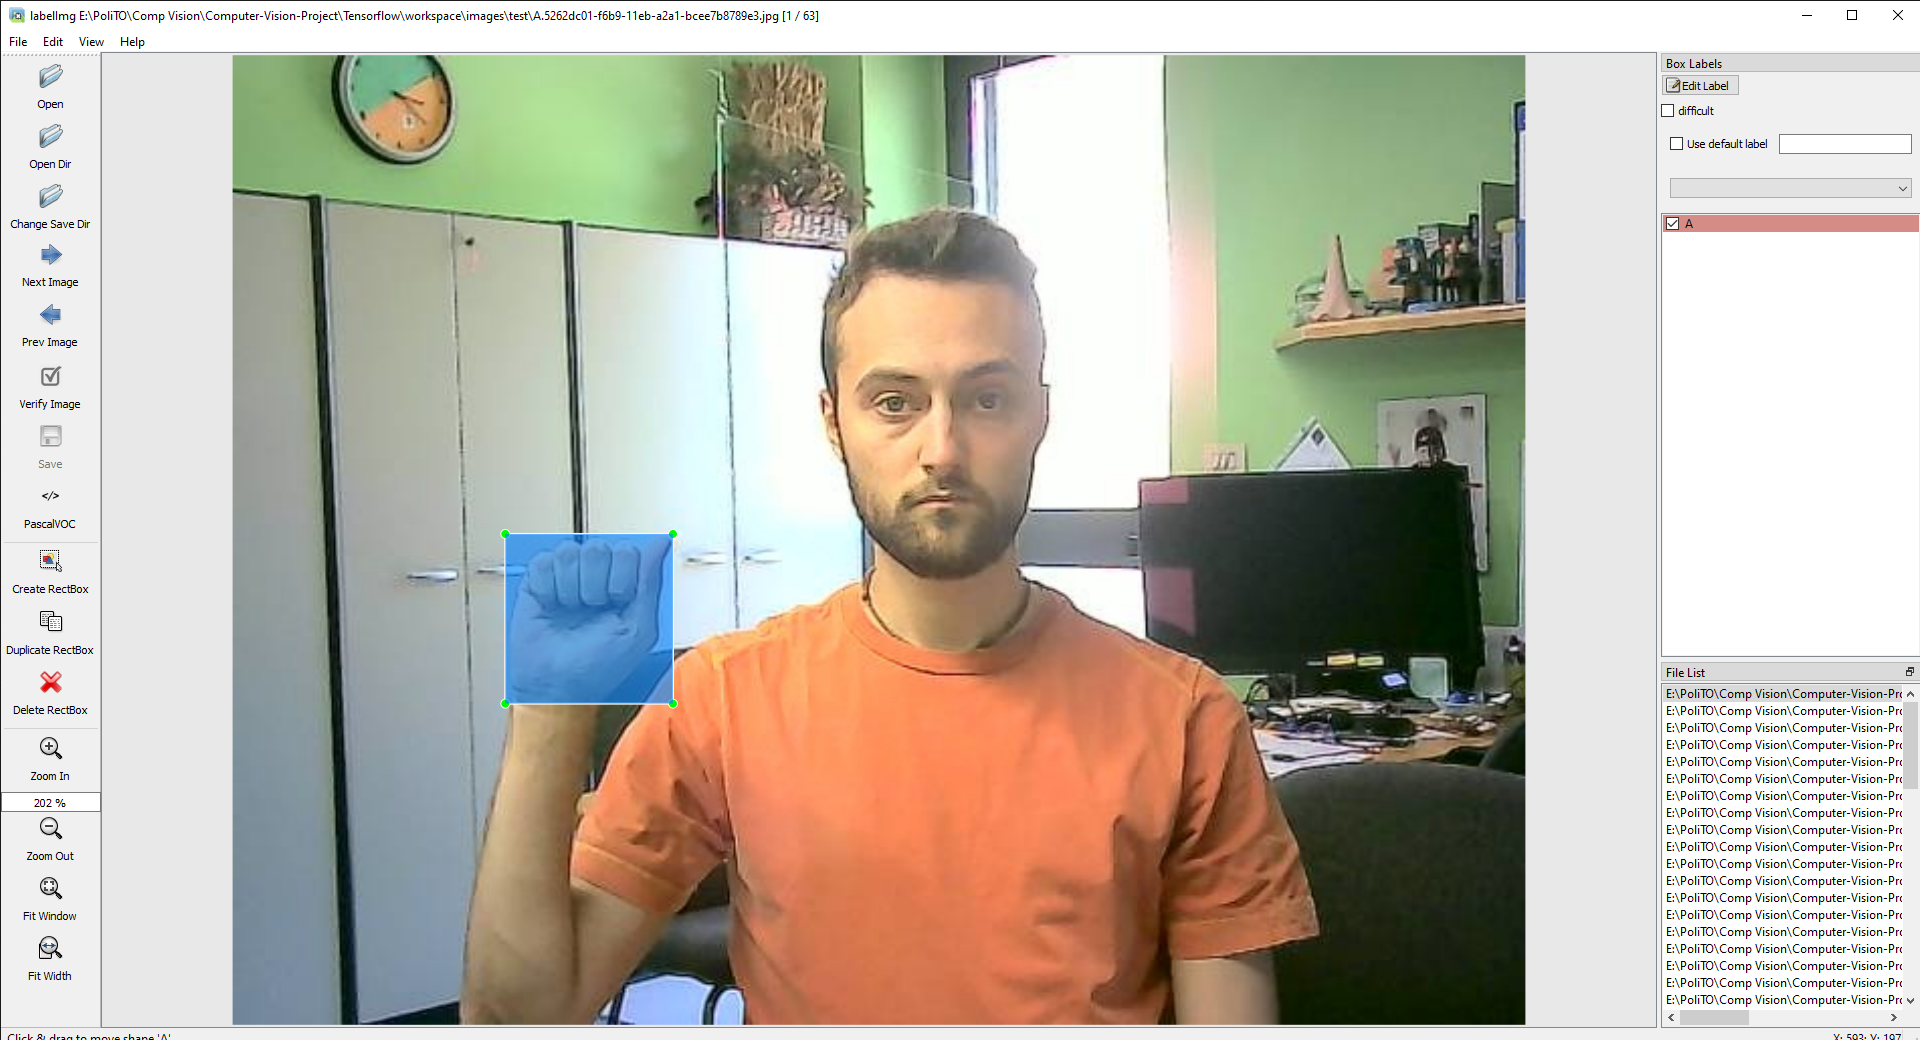
\includegraphics[width=0.5\textwidth]{resources/image/labelImgScreenshot.PNG} \caption{The LabelImg interface after drawing a bounding box around the \textit{A} gesture.}
\end{figure}

\subsection{Neural network training}
\label{NeuralNetworkTraining}
Once the dataset has been labeled we can train the neural network.
To do so we have to split the dataset into two parts, one to be used for training and the other for testing. It's important to note that each frame must be moved alongside its corresponding \textit{.xml} file.\linebreak
The following steps are also described in the Python Notebook \href{https://github.com/MarzioVallero/Real-time-Sign-Language-Detection/blob/master/LabelDatasetAndTrain.ipynb}{LabelDatasetAndTrain.ipynb}.\linebreak
We create a Label Map for the different labels in the dataset, then embed all the the \textit{.xml} files associated to each frame to two \textit{.record} files, \textit{train.record} and \textit{test.record}, a specific file format necessary to interface a datset with Tesorflow. \linebreak
Trainig and testing is automated through \textit{\hyperref[Ref9]{Tensorflow's Object Detection API}}, a free open source software library for machine learning focused on object recognition.\linebreak
The training technique involves transfer learning from a general purpose pre-trained model, the \textit{SSD MobileNet V2 FPNLite 320x320}, a Single Shot MultiBox Detector Feature Pyramid Network, which is available from \textit{\hyperref[Ref10]{Tensorflow's Detection Model Zoo}}, trained on the \textit{\hyperref[Ref2]{COCO dataset}}. We chose this network as we needed a very fast Box based detection network with sufficient accuracy, and it is, with a detection speed of $22 ms$ on average and a COCO mAP score of $22.2$.
Other pre-trained models lacked in one or more of the desired characteristics and were thus ultimately discarded as candidates for our project.\linebreak
The SSD's approach is different from other object detection system that usually follow these steps: assume bounding boxes, resample pixels or features for each box, and apply a high quality classifier, repeating the step for a fixed number of iterations. With this approach there is a fundamental improvement in terms of speed because bounding box proposal is deleted, as well as the subsequent phase of pixel or feature resampling, and all computation is encapsulated in a single network, as seen in the \textit{\hyperref[Ref1]{Single Shot MultiBox Detector paper}}.     
The training process is thus sped up through transfer learning from the SSD FPN to the final network trained on our custom image set. With this technique, the final model boasts high accuracy despite using a reduced dataset, cutting down on time requirements for labeling and training. The main principle which allows the trasfer of knowledge across different but related source domains is the idea of generalization of experience, as illustrated in the \textit{\hyperref[Ref3]{Comprehensive Survey on Transfer Learning}}.

\subsection{Gaze recognition}
\label{GazeRec}
Whilst developing the project, we noticed that the program had no way to recognize willingness of a gesture: this ultimately lead to gestures being detected also when the user wasn't intentionally interacting with the application. For this reason we introduced a gaze detection algorithm based on the trained deep neural network \textit{\hyperref[Ref12]{Faster RetinaFace}} provided as an improvement on the provided alongside the \textit{\hyperref[Ref4]{RetinaFace: Single-ShotMulti-Level Face Localisation in the Wild}} paper.
The Gaze recognition portion of the software is based on a cascade approach at different levels of granularity to effectively increase detection speed.
The first layer of the algorithm employs the \textit{\hyperref[Ref12]{Faster RetinaFace}}, used to detect the regions of interest in the frame containing a face. This step, as opposite to the Haar cascade used for masking, is extremely precise and allows for detection of faces at variable positions and rotations.\linebreak
Each region of interest is then processed by applying the \textit{\hyperref[Ref13]{Deep Face Alignment}} process, using the  stacked Hourglass heatmap based approach for robust 2D and 3D face alignment. The topology of the deep face alignment layer is built with alignment network multi-scale (HPM) residual block and channel aggregation blocks (CAB).
The topology of the deep face is sent to the \textit{\hyperref[Ref14]{Head Pose Estimation}} which applies cascaded regression trees to predict the face's shape (i.e. feature locations) change in every frame. Splitting nodes of trees are trained in random, greedy, maximizing variance reduction fashion. This step produces a point cloud representing the feature locations of the detected face.\linebreak
The feature locations are used to pinpoint the orientation of the segmented iris with respect to the eye's position according to the \textit{\hyperref[Ref7]{Realtime and Accurate 3D Eye Gaze Capture with DCNN-Based Iris and Pupil Segmentation}} paper.
The iris position and face alignment are then used to compute the gaze direction of the user, producing two 2D vectors with origin at the iris's center and pointing towards the approximate gaze direction of the detected face.\linebreak
The norm of the two gaze vectors equals zero when the user stares directly into the camera and grows as he or she looks further away from it: it has thus been used as the decision metric to separate frames in which the user is looking towards the screen from in which it's not doing so.

\subsection{Real time sign language detection}
\label{RTSignDetect}
The previously trained model is thus used to detect hand signs in image frames, however we must try to reduce input error as much as possible.
During the initial testing phase, we noticed that the trained model had some difficulties in correctly identifying the hand due to the detection noise from the background other objects and varaible ambient illumination during the day or from different angles. We thus applied a first step consisting in a double masking approach: the frame is HSV thresolded for skin-toned pixels, then an Haar cascade detection algorithm is used to detect a bounding box for the faces in the frame and removing them.\linebreak
However, variable illumination conditions and skin tones required a broader HSV filter, which still let trough too much noise. In order to address this issue, we included an additional \textit{\hyperref[https://github.com/MarzioVallero/Real-time-Sign-Language-Detection/blob/master/CreateHSVProfile.py]{interactive script CreateHSVProfile.py}}, available also in Notebook form, that lets the user create a custom HSV thresolding profile, which are automatically saved in a configuration file \textit{config.dat} and loaded in by the \textit{\hyperref[https://github.com/MarzioVallero/Real-time-Sign-Language-Detection/blob/master/SignDetection.py]{SignDetection.py}}. If no config.dat file is found, a temporary dictionary with statistically relevant default values is used instead.\linebreak
The gaze detection network is then fed with the original not-masked frame input, producing two 2D eye gaze direction vectors, on for each eye. If the norm of the gaze vectors is collectively smaller than a certain threshold, it means that the user is looking towards the camera. If the user looks away for more than five consecutive frames, or no user is detected, the sign detection is suspended until a user looking towards the camera is detected again.\linebreak
If the gaze detection step is passed, the sign detection neural network is invoked, passing as argument the previously masked frame. The network outputs a structure, containing an array of tuples (label, accuracy) and other arrays, alongside which one accounts for the bounding box coordinates of each detected sign.\linebreak
If a gesture is kept stable for five frames, it's added to the output string buffer. In order to improve the software's input capabilities, specific temporal combinations of basic signs have been set up to be recognized as special actions to be used as additional means of interaction. This reduces the stress on the neural network's side, reducing the chance of sign prediction error, other than avoiding the addition of extra non-standard gestures for the user to learn. The sign combinations have been chosen to be easy to perform and logically coherent with the action they represent.\linebreak
At last, the resulting output and string buffer are displayed on a window through the \textit{matplotlib} python library.

\section{Results and Analysis}
\label{ResutsAndAnalysis}
The result of our work is a software capable of detecting in real time the Italian Sign Alphabet [figure \ref{fig:sign}] if it actively finds a user trying to interact with it. It accomplishes its goal of being a reliable mean of interaction, as the user can input any character plus and additional set of special actions.\linebreak
The currently provided network is a right hand trained model, able to recognize static gestures. Using left-handed gestures may incur in aliasing problems.
\begin{figure}[!h]
    \centering
    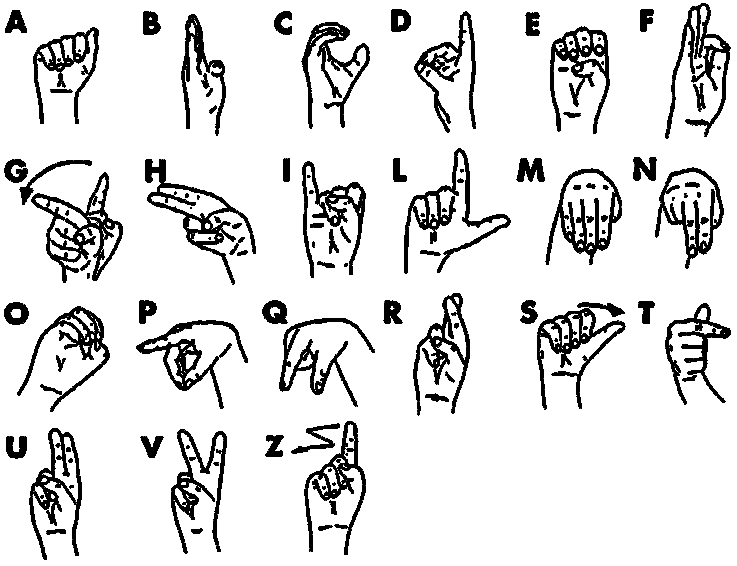
\includegraphics[width=0.5\textwidth]{resources/image/sign.png} \caption{The characters in the standard Italian alphabet.} \label{fig:sign}
\end{figure}

On a performance standpoint, it must be noted that the neural network portion of the software is the most computationally intensive and as such, should be run on dedicated CUDA enabled GPUs.\linebreak
In our case, since we did not have a CUDA enabled GPU available for accelerating the detection, it has been instead run on the CPU: as such, this impacted the final performance in output frames per second. On the other hand though, the current configuration of the project be run on any machine with a powerful enough consumer CPU.\linebreak
In our case, a \textit{Intel i7-4770} was able to output up to 10-12 frames per second when both the Gaze Detection network and the Sign Detection networks were running together, and up to 25-30 frames per second when only the Sign Detection network was running.\linebreak

\section{Usage}
\label{Usage}
The following guide takes as granted that a user is detected in the frame and is looking towards the camera.\linebreak
When a character is detected, a bounding box surrounds the hand gesture in the frame, displaying the detected sign's label as feedback and the detection accuracy score as a percentage [figure \ref{fig:letter}].\linebreak
All detected signs with detection accuracy lower than $70\%$ are ignored and, in any case, no more than one bounding box is displayed per frame, although more than one sign in usually detected: this is done as a measure to reduce as much as possible user-perceived aliasing.\linebreak

\begin{figure}[!h]
    \centering
    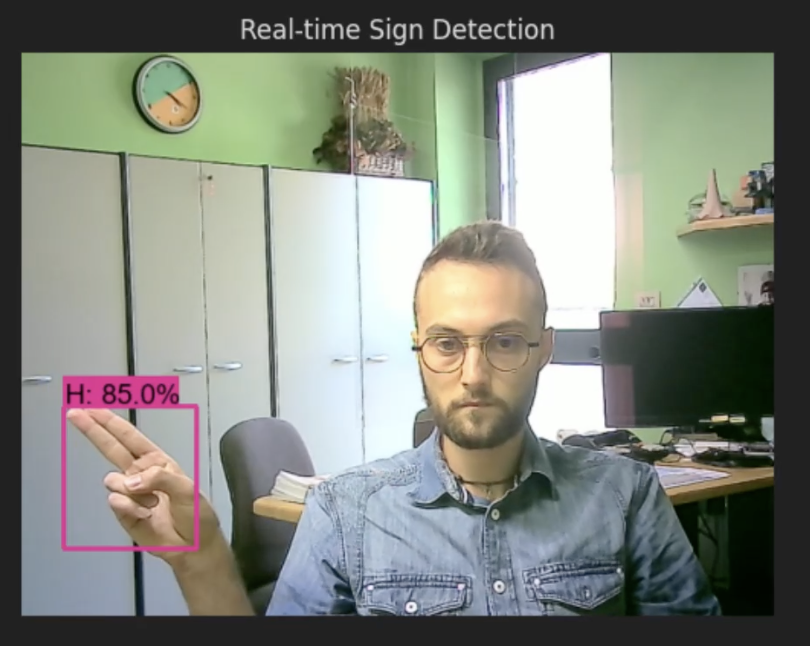
\includegraphics[width=0.5\textwidth]{ComputerVisionReport/resources/image/letter.png} \caption{Letter H has been detected.} \label{fig:letter}
\end{figure}

When a sign is held stable for five frames, the corresponding letter is stored in a string buffer and shown on screen, in order to provide additional feedback to the user [figure \ref{fig:print}].\linebreak

\begin{figure}[H]
    \centering
    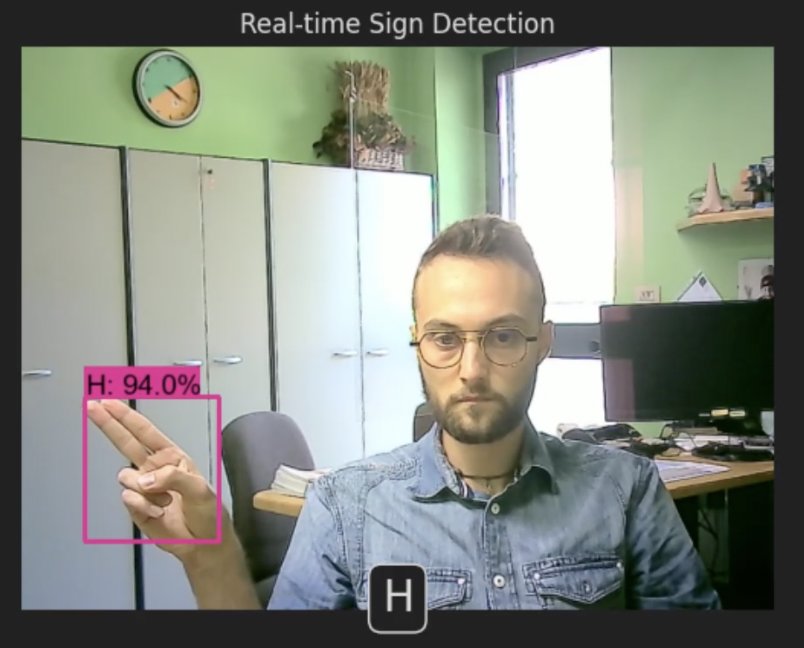
\includegraphics[width=0.5\textwidth]{ComputerVisionReport/resources/image/print.png} \caption{Letter H displayed on screen.} \label{fig:print}
\end{figure}

As stated in the previous section, special temporal gestures have been introduced in order to let the user perform high level interaction with the software. These special gestures are registered as specific couples of characters detected in quick succession:\linebreak
\begin{itemize}
\item An "A" gesture followed by an "S" gesture, appends a space to the active string buffer.
\item A "V" gesture followed by a "U" gesture, deletes the last character in the active string buffer.
\item An "E" gesture followed by an "A" gesture, deletes all the characters in the active string buffer.
\item A "D" gesture followed by an "O" gesture, prints the active string buffer to stdout, then deletes all the characters in the active string buffer.
\end{itemize}

\begin{figure}[!h]
    \centering
    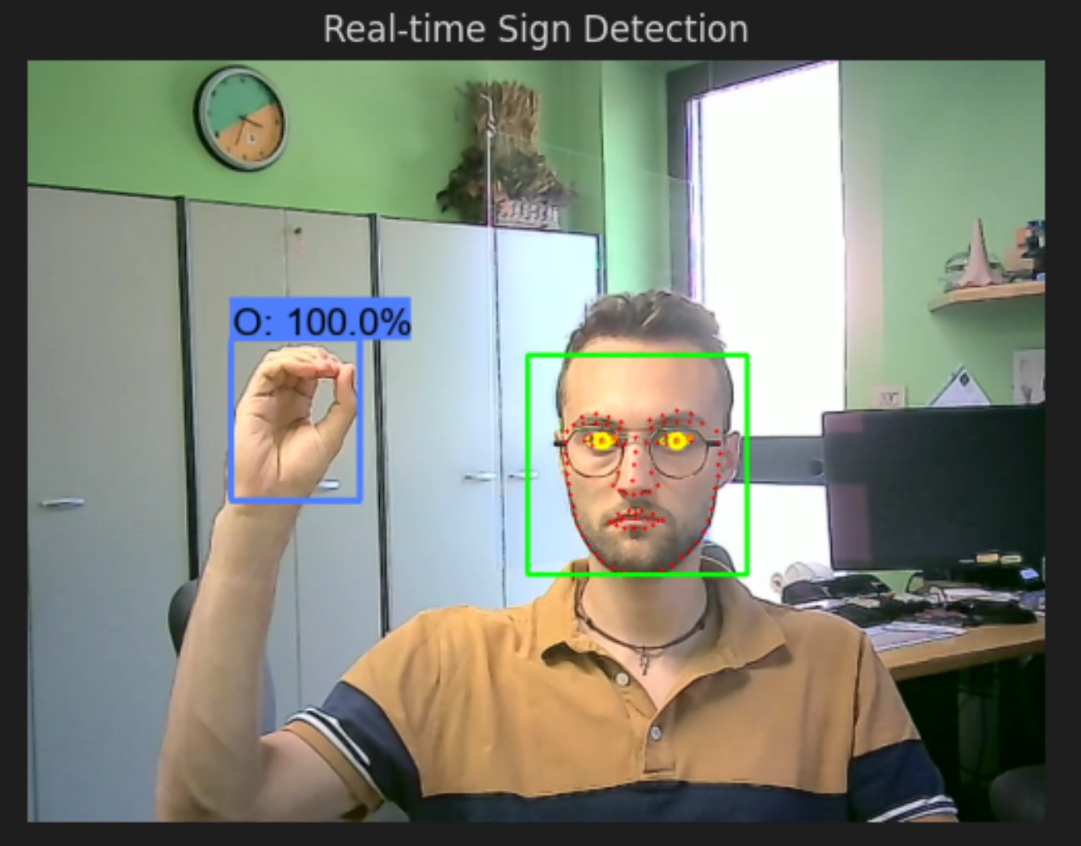
\includegraphics[width=0.5\textwidth]{ComputerVisionReport/resources/image/DebugO.PNG} \caption{The frame with all features printed on screen. The gaze vectors have norm almost zero, thus are drawn as orange dots.}
\end{figure}

Running the script with the \textit{--Debug} option, gives the user the possibility to enter a debug mode which allows the person to see every landmark used by the program to process the face and the eyes movement, as well as the gaze direction vectors.\linebreak
The green bounding box represents the face detection performed by the Haar classifier and is used for masking purposes: since after HSV skin-tone thresholding the face is still visible, sometimes certain parts of the face could be recognized as signs.\linebreak
The facial landmarks are drawn as red dots, the pupils are highlighted with yellow circles and the gaze direction vectors are printed as arrowed lines in orange.

\begin{figure}[!h]
    \centering
    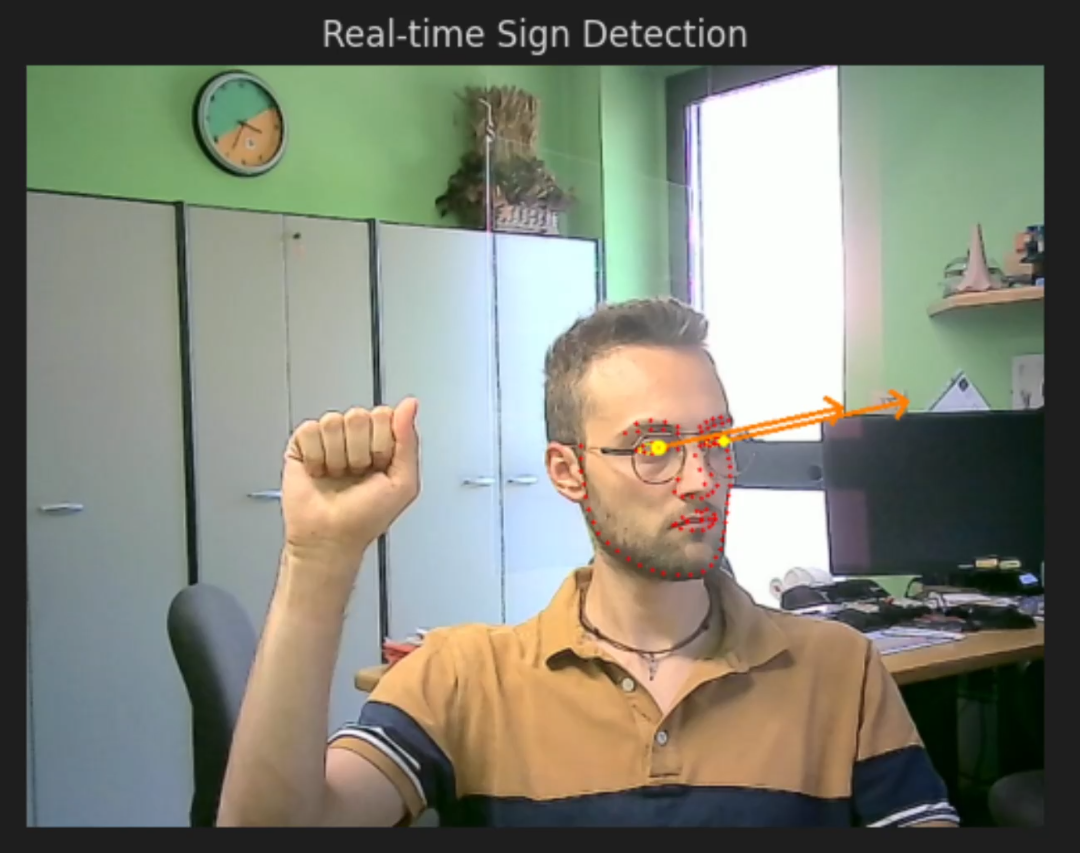
\includegraphics[width=0.5\textwidth]{ComputerVisionReport/resources/image/DebugANotLooking.PNG} \caption{The user is looking away, thus the \textit{A} sign is ignored.}
\end{figure}


\section{Conclusions}
\label{Conclusions}
During development, we stumbled upon multiple issues.
Various object classifiers didn't provide the expected results, such as Haar’s Classifiers for eyes recognition, or were too unstable.
Tensorflow's APIs, being extremely vast required a lot of know-how to be setup properly. In order to produce a working model with sufficient accuracy, multiple datasets and training sessions had to be done.
For gaze detection, multiple segmentation algorithms have been tried before finding an approach that suited our needs.\linebreak
However, we refused to stop and kept on trying.
At the end of development, we were glad of what we had accomplished. We understood that Computer Vision can pave the way for better means of interaction between humans and machines.\linebreak
We hope that machines will have the chance to improve humanity's tomorrow.

\section{Acknowledgments}
\label{Acks}
The project has been developed for the Computer Engineering Masters Degree exam Image Processing and Computer Vision, taught by professors B. Montrucchio and L. De Russis, during the a.y. 2020/2021 at the Polythecnic of Turin.

\onecolumn
\section{References}
\label{References}
\begin{flushleft}
\begin{itemize}
    \item \label{Ref1} \href{https://arxiv.org/abs/1512.02325}{Liu W., Anguelov D., Erhan D., Szegedy C., Reed S., Fu C., Berg A. C.: Single Shot MultiBox Detector}. 2016.
    \item \label{Ref2} \href{https://arxiv.org/abs/1405.0312}{Lin T., Maire M., Belongie S., Bourdev L., Girshick R., Hays J., Perona P., Ramanan D., C. Zitnick L., Dollár P.: Microsoft COCO: Common Objects in Context}. 2015.
    \item \label{Ref3} \href{https://arxiv.org/abs/1911.02685}{Zhuang F., Qi Z., Duan K., Xi D., Zhu Y., Zhu H., Xiong H., He Q.: A Comprehensive Survey on Transfer Learning}. 2020.
    \item \label{Ref4} \href{https://openaccess.thecvf.com/content_CVPR_2020/html/Deng_RetinaFace_Single-Shot_Multi-Level_Face_Localisation_in_the_Wild_CVPR_2020_paper.html}{ Deng J., Guo J., Ververas E., Kotsia I., Zafeiriou S.: RetinaFace: Single-Shot Multi-Level Face Localisation in the Wild}. 2020.
    \item \label{Ref5} \href{https://ieeexplore.ieee.org/document/1195992}{Ansar A., Daniilidis K.: Linear pose estimation from points or lines}. 2003.
    \item \label{Ref6} \href{https://openaccess.thecvf.com/content_cvpr_2017/html/Ke_An_Efficient_Algebraic_CVPR_2017_paper.html}{ Ke T., Roumeliotis S.I.: An Efficient Algebraic Solution to the Perspective-Three-Point Problem}. 2017.
    \item \label{Ref7} \href{https://ieeexplore.ieee.org/document/8818661}{Wang Z., Chai J., Xia S.: Realtime and Accurate 3D Eye Gaze Capture with DCNN-Based Iris and Pupil Segmentation}. 2021.
    \item \label{Ref8} \href{https://tensorflow-object-detection-api-tutorial.readthedocs.io/en/latest/}{Tensorflow Object Detection API installation}
    \item \label{Ref9} \href{https://github.com/tensorflow/models/tree/master/research/object_detection}{Tensorflow Object Detection API GitHub}
    \item \label{Ref10} \href{https://github.com/tensorflow/models/blob/master/research/object_detection/g3doc/tf2_detection_zoo.md}{TensorFlow 2 Detection Model Zoo}
    \item \label{Ref11} \href{https://github.com/tzutalin/labelImg}{LabelImg GitHub}
    \item \label{Ref12} \href{https://github.com/1996scarlet/faster-mobile-retinaface}{Faster RetinaFace}
    \item \label{Ref13} \href{https://github.com/deepinx/deep-face-alignment}{Deep Face Alignment}
    \item \label{Ref14} \href{https://github.com/lincolnhard/head-pose-estimation}{Head Pose Estimation}
\end{itemize}
\end{flushleft}

\end{document}